\begin{spacing}{1.5}
  \begin{tightcenter}
    \section{1. Introducción}
    \mylinespacing
  \end{tightcenter}

  El objetivo de la tesis presentada es maximizar la utilización de los
  recursos disponibles en el clúster Bochica y la sala de cómputo Jürgen Tischer
  del departamento de Matemáticas de la Universidad del Valle. A pesar de contar
  con una cantidad considerable de medios computacionales, estos recursos no
  están siendo utilizados de manera óptima. Para abordar este problema, se
  propone una metodología que consiste en la implementación de un gestor de cola
  de tareas con capacidades de paralelización, lo que permitirá una utilización
  más eficiente y efectiva de los recursos en investigaciones matemáticas.

  Para alcanzar este objetivo, se propone utilizar sistemas distribuidos como
  estrategia para aprovechar al máximo los recursos disponibles. Estos sistemas
  permiten la paralelización de tareas y la distribución de la carga de trabajo
  entre varios nodos o dispositivos, lo que implica la posibilidad de aprovechar
  la capacidad total de cómputo de los recursos disponibles. Además, estos
  sistemas ofrecen una mayor flexibilidad y escalabilidad en el uso de los
  recursos, lo que resulta esencial en un entorno de investigación matemática
  donde las necesidades de cómputo pueden variar significativamente.

  Se realizará un análisis de diversos programas informáticos en esta tesis con
  el fin de proponer una implementación específica de un sistema distribuido que
  permita un mayor rendimiento y eficiencia en comparación con otros métodos
  existentes. Además, se evaluará el desempeño del sistema propuesto en relación
  con otros métodos, para determinar su efectividad en la optimización del uso de
  los recursos disponibles en el clúster Bochica y la sala de computación Jürgen
  Tischer.

  \subsection{1.1 Planeamiento del problema}

  \textbf{Descripción del problema}

  La falta de acceso a capacidades computacionales adecuadas está limitando la
  capacidad de los trabajos relacionados con la investigación, análisis de datos
  y simulación de procesos en el campo de la Ciencias en la Universidad del
  Valle. Esto se ha reflejado en un enfoque predominantemente teórico en lugar de
  computacionalmente intenso en estos trabajos de investigación. El Departamento
  de Matemáticas identifica esta limitación como un problema y ve la necesidad de
  acceder a recursos computacionales más potentes para poder llevar a cabo
  cálculos matemáticos a gran escala con fines investigativos.

  \textbf{Formulación del problema}

  ¿Cómo podrían satisfacerse las demandas de cómputo requeridas para la
  investigación matemática utilizando los recursos disponibles de manera
  eficiente? ¿Cómo se podría facilitar el acceso y uso de estos recursos para que
  puedan ser utilizados por la comunidad universitaria sin necesidad de
  conocimientos técnicos avanzados?

  \subsection{1.2 Justificación del problema}

  \textbf{Justificación Académica}

  La posibilidad de contar con una capacidad de procesamiento a gran escala con
  capacidades de paralelización representa una oportunidad para ampliar el
  alcance de la investigación científica en la Universidad, no solo en el ámbito
  de las matemáticas sino también en otras disciplinas científicas.

  \textbf{Justificación Económica}

  Aunque existen opciones similares a las propuestas en este trabajo, como
  servicios de computación en la nube, suelen carecer de accesibilidad económica
  para estudiantes y profesores investigadores. En este sentido, el presente
  proyecto tiene como objetivo aprovechar recursos subutilizados dentro de la
  Universidad del Valle, con el fin de maximizar su potencial y hacerlos
  accesibles para la comunidad universitaria, ahorrando así en la inversión de
  nuevos equipos y recursos.

  \textbf{Justificación Social}

  La disponibilidad de un recurso propio y de bajo costo contribuiría a la
  democratización del acceso a plataformas de alto rendimiento o masivamente
  paralelas, lo que podría aumentar la inclusión de estudiantes, profesores e
  investigadores de diferentes disciplinas en el ámbito de la investigación y el
  desarrollo científico.

  \subsection{1.3 Objetivos}

  \textbf{Objetivo general}

  La presente tesis tiene como objetivo desarrollar un servicio de computación
  con capacidades de paralelización, el cual estará disponible para la comunidad
  universitaria y se enfocará en apoyar la investigación en el ámbito académico.
  Para lograr esta meta, se propone aprovechar los recursos existentes en el
  Departamento de Matemáticas de la Universidad del Valle. Este servicio busca
  optimizar el uso de los recursos informáticos y permitir una mayor eficiencia
  en el procesamiento de datos, mejorando así las posibilidades de investigación
  y contribuyendo al avance de la comunidad académica en general.

  \textbf{Objetivos específicos}
  \begin{enumerate}
    \item Identificar recursos disponibles y necesidades investigativas.
    \item Diseñar una solución que considere los requerimientos de los usuarios
          y aproveche las capacidades de los recursos computacionales mediante la
          implementación de un gestor de cola de tareas.
    \item Llevar a cabo la instalación, documentación y puesta a punto de
          herramientas que apoyen los procesos de investigación y docencia en el área de
          matemáticas, facilitando el uso del servicio.
    \item  Llevar a cabo pruebas de uso de la infraestructura y de las
          aplicaciones desplegadas en este trabajo.\newline
  \end{enumerate}

  \subsection{1.4 Estado del arte}

  Desde sus orígenes, la informática y la computación han estado íntimamente
  relacionadas con las matemáticas. En la actualidad, la capacidad para realizar
  cálculos y análisis de datos a gran escala resulta fundamental en numerosos
  campos de investigación científica. Sin embargo, en la Universidad del Valle se
  ha identificado una limitación en el acceso a estas capacidades
  computacionales, lo que ha ocasionado que los trabajos de investigación se
  centren principalmente en enfoques teóricos, en lugar de los enfoques
  computacionalmente intensivos. Es importante señalar que este problema no solo
  afecta al Departamento de Matemáticas, sino también a otras áreas de
  investigación de la universidad.

  Para abordar esta problemática, resulta crucial considerar el estado actual
  del arte en cuanto a la disponibilidad de recursos informáticos para la
  investigación. Es importante aclarar que los recursos informáticos a considerar
  en el análisis tienen que ver con software, ya que este es esencial para llevar
  a cabo cálculos y análisis de datos a gran escala. Es necesario evaluar
  cuidadosamente las opciones existentes, teniendo en cuenta la viabilidad de
  cada alternativa dentro del contexto de la Universidad del Valle.

  Adicionalmente, es de vital importancia indagar acerca de las mejores
  prácticas y estrategias empleadas por otras instituciones y organizaciones para
  abordar problemáticas similares. En este sentido, es posible analizar
  experiencias exitosas en la implementación de soluciones informáticas efectivas
  para la investigación.

  En primer lugar, exploraremos el concepto de computación distribuida y,
  posteriormente, analizaremos proyectos que emplean este enfoque con el fin de
  alcanzar resultados similares a los objetivos que se persiguen en el presente
  proyecto.

  \subsubsection{1.4.1 Computación Distribuida}

  La computación distribuida es un enfoque de procesamiento de datos en el que
  múltiples computadoras se utilizan en conjunto para realizar tareas de cómputo
  complejas de manera coordinada y en paralelo. En lugar de tener una sola
  computadora realizando todos los cálculos, la carga de trabajo se distribuye
  entre muchas computadoras que trabajan en paralelo para resolver el problema
  más rápidamente.

  \begin{figure}[h]
    \centering
    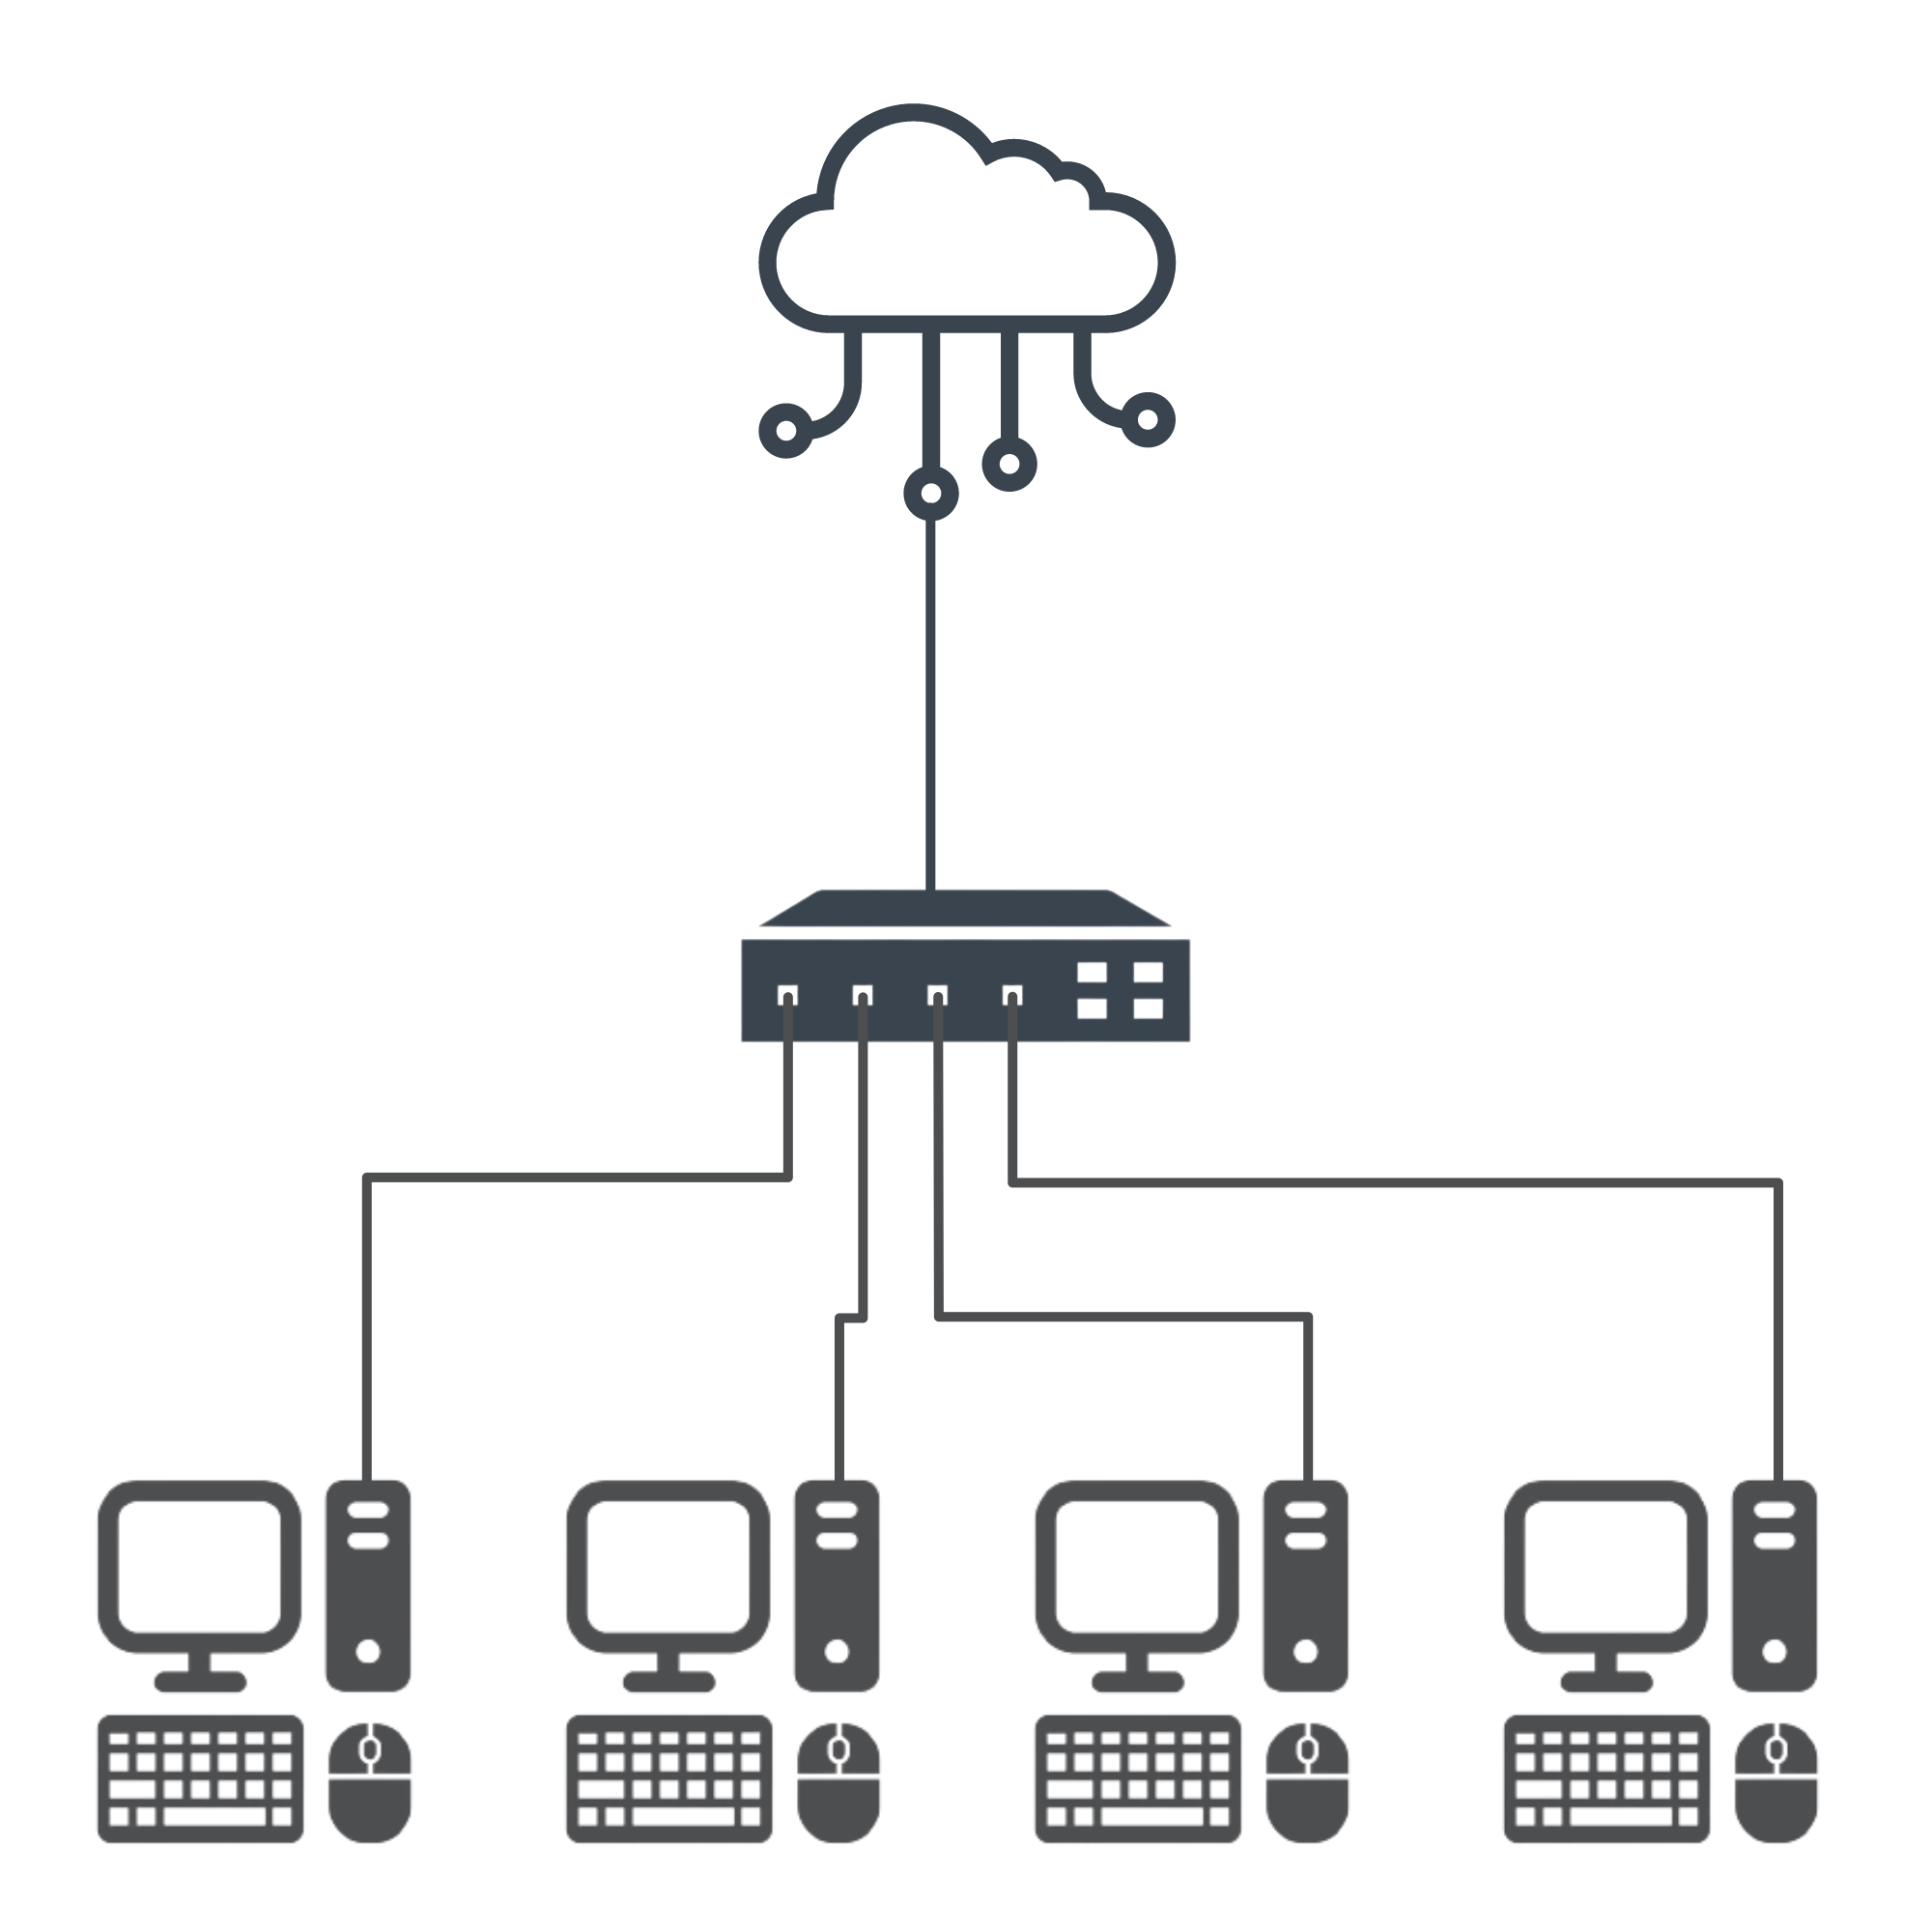
\includegraphics[width=0.5\textwidth]{ds.png}
    \caption{Sistema Distribuido}
    \label{fig:etiqueta}
  \end{figure}

  Este enfoque es particularmente útil para resolver problemas que requieren
  grandes cantidades de datos o cálculos intensivos, como la simulación de
  sistemas complejos, el procesamiento de imágenes y video, y la modelización de
  sistemas físicos o biológicos.

  Para implementar la computación distribuida, se requiere conectividad de
  redes de alta velocidad, lo que permite a las computadoras comunicarse y
  coordinarse para realizar tareas de forma colaborativa. A menudo, se utilizan
  software y protocolos especializados para coordinar y administrar el
  procesamiento distribuido, asegurando que las tareas se asignen y se completen
  de manera efectiva.

  En general, la computación distribuida puede resolver problemas complejos en
  tiempos asequibles, ya que permite que una gran cantidad de recursos de
  procesamiento se utilicen en paralelo para acelerar el procesamiento. Además,
  la computación distribuida también puede hacer posible que se aborden problemas
  que serían demasiado costosos o imposibles de abordar mediante el uso de una
  única computadora o servidor. \cite{distributed-1}, \cite{distributed-4},
  \cite{distributed-3}

  \subsubsection{1.4.2 Tipos de Sistemas Distribuidos}

  Los sistemas distribuidos constituyen una categoría de sistemas que emplean
  una serie de dispositivos que colaboran para llevar a cabo una tarea en
  particular. Estos sistemas pueden intercomunicarse de diferentes formas y
  enfrentar distintos tipos de problemas.

  Existen diversas formas en las que los sistemas distribuidos pueden
  comunicarse y resolver problemas, cada una con sus ventajas y desventajas
  dependiendo del contexto en el que se apliquen. Sin embargo, para los fines de
  este proyecto, nos centraremos en los tipos de sistemas distribuidos HPC y HTC.
  \vspace{3mm}

  \textbf{HPC(High Performance Computing)}

  Entre los tipos de sistemas distribuidos más notables, se encuentra el HPC,
  que se enfoca en la ejecución de tareas que demandan una alta capacidad de
  procesamiento. Se utiliza en campos como la investigación científica, el diseño
  de productos y el análisis financiero, entre otros.

  \textbf{HTC (High Throughput Computing)}

  Otro tipo de sistema distribuido es el HTC, que se centra en realizar
  numerosas tareas en un tiempo de respuesta reducido. Se emplea en áreas como la
  bioinformática, la simulación de procesos industriales y la creación de
  contenido multimedia.
  A lo largo del tiempo, han surgido diversas soluciones de software para hacer
  frente a la complejidad que conlleva el uso de sistemas distribuidos. Entre las
  soluciones más destacadas y relevantes para este proyecto se encuentran SLURM,
  que utiliza HPC, y HTCondor, basado en HTC.  \vspace{3mm}

  \textbf{SLURM Y HTCondor}

  A partir de las dificultades inherentes a la utilización de sistemas
  distribuidos, se han desarrollado diversas soluciones de software. En el marco
  de este proyecto, se consideran pertinentes dos de los más populares gestores
  de cola de tareas: SLURM y HTCondor, ambos sistemas tienen enfoques diferentes
  en términos de diseño y funcionalidad. SLURM está diseñado principalmente para
  clústeres de computación de alta velocidad y está optimizado para la gestión de
  trabajos de paralelización de tareas computacionales. Por otro lado, HTCondor
  es un sistema de gestión de recursos más general que puede manejar sistemas
  heterogéneos y distribuidos, incluidos los recursos de la nube y las redes
  internacionales.

  \textbf{SLURM (Simple Linux Utility for Resource Management)}

  SLURM es un sistema de gestión de recursos de código abierto para clústeres
  de computadoras de alto rendimiento (HPC) en entornos de sistemas distribuidos.
  SLURM es utilizado por numerosas instituciones académicas, gubernamentales y
  comerciales para gestionar y programar trabajos de computación en clústeres de
  Linux de diferentes tamaños, desde pequeños clústeres universitarios hasta
  grandes supercomputadoras. \cite{DEF-SLURM}

  Este gestor de cola de tareas se centra en la gestión de tareas de
  procesamiento de alta velocidad y de alto rendimiento, como la simulación, la
  modelización, la genómica, la bioinformática, la física y la ingeniería.
  Permite la ejecución eficiente de trabajos paralelos y distribuidos en
  clústeres de HPC y utiliza un enfoque modular que permite una configuración
  personalizada para satisfacer las necesidades específicas de cada clúster.

  \begin{figure}[h]
    \centering
    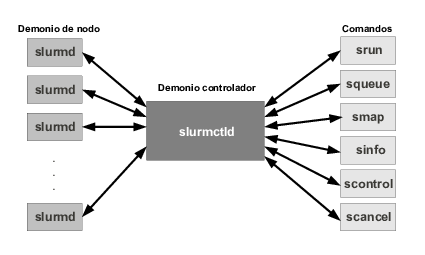
\includegraphics[width=0.5\textwidth]{as.png}
    \caption{Arquitectura SLURM}
    \label{fig:etiqueta}
  \end{figure}

  SLURM utiliza un modelo de cola de trabajos para administrar y priorizar
  trabajos en el clúster. Los trabajos se envían a la cola y se programan
  automáticamente para ejecutarse en los nodos del clúster disponibles según las
  especificaciones del usuario. SLURM también proporciona herramientas para la
  monitorización del clúster, la gestión de usuarios y grupos, la gestión de
  recursos y el seguimiento del estado de los trabajos en
  ejecución.\cite{DOC-SLURM}
  \vspace{3mm}

  \textbf{HTCondor (High Throughput Computing Condor)}

  HTCondor es un sistema de software de código abierto que se utiliza para la
  gestión y programación de trabajos de alta capacidad en entornos de computación
  de alto rendimiento. Este sistema permite la utilización efectiva de la
  potencia de cálculo de máquinas conectadas en una red, ya sea un único clúster,
  un conjunto de clústeres en un campus, recursos en la nube independientes o
  unidos temporalmente a un clúster local, o redes internacionales.
  \cite{DOC-HTCONDOR}

  HTCondor es conocido por su capacidad para gestionar sistemas heterogéneos y
  distribuidos, lo que lo hace especialmente adecuado para entornos en los que se
  utilizan diferentes sistemas operativos y arquitecturas de hardware. Se utiliza
  en muchos campos, incluyendo la investigación académica, la física, la
  ingeniería, la biología y la industria.

  \begin{figure}[h]
    \centering
    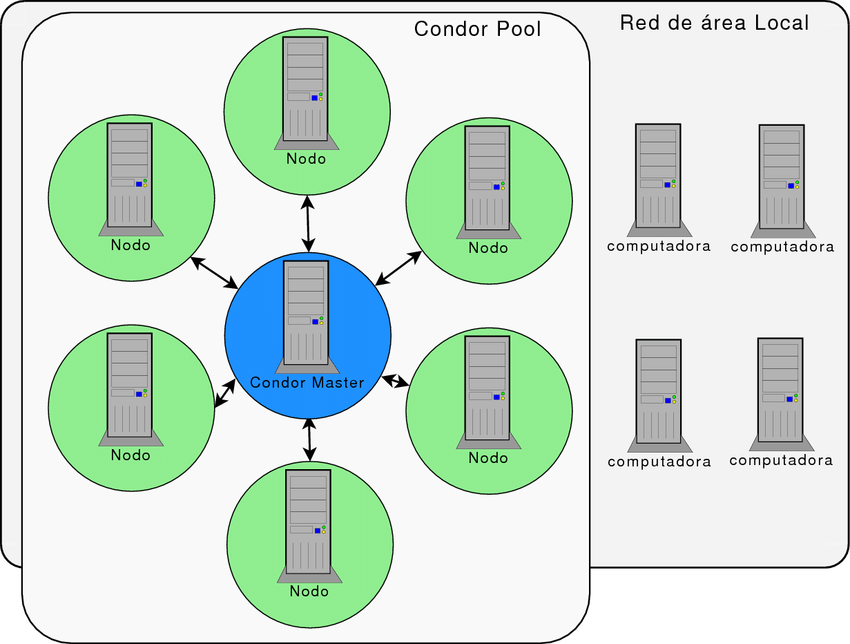
\includegraphics[width=0.5\textwidth]{ah.png}
    \caption{Arquitectura centralizada del entorno Condor.}
    \label{fig:etiqueta}
  \end{figure}

  Este sistema utiliza un modelo de cola de trabajos que permite a los usuarios
  enviar trabajos a la cola y programarlos para que se ejecuten en el momento
  adecuado y en los nodos adecuados del clúster. Además, proporciona herramientas
  para la monitorización del clúster, la gestión de usuarios y grupos, la gestión
  de recursos y el seguimiento del estado de los trabajos en ejecución.
  \cite{DEF-HTCONDOR}

  \subsubsection{1.4.3 Computación distribuida en proyectos similares}

  En esta sección del estado del arte, se presentarán algunos proyectos que
  utilizan la computación distribuida como herramienta en la resolución de
  problemas complejos. La revisión de proyectos previos es una parte esencial del
  proceso de investigación, ya que permite identificar qué se ha investigado en
  el pasado y qué se ha logrado hacer.

  Los proyectos que se presentarán a continuación han sido seleccionados por su
  relevancia en los diferentes tipos de sistemas distribuidos existentes, que
  resulta una parte fundamental de la investigación que se lleva a cabo en esta
  tesis. Cada proyecto se describirá brevemente, destacando sus principales
  objetivos, metodologías y resultados.

  El análisis de proyectos similares es importante para contextualizar la
  investigación actual en el campo de estudio y para identificar qué áreas aún
  necesitan ser exploradas. Con esta revisión, se espera proporcionar un marco de
  referencia útil para la investigación actual y, en última instancia, mejorar la
  comprensión de los desafíos y las oportunidades en el campo.

  \textbf{PL-Grid (Polonia)}

  PL-Grid es un proyecto polaco que tiene como objetivo principal proporcionar
  una infraestructura de computación distribuida de alta capacidad a partir de
  recursos heterogéneos con interfaz unificada que permita el fácil acceso a la
  infraestructura informática distribuida a gran escala para apoyar la
  investigación científica y académica. La red es gestionada por el Consorcio
  Interdisciplinario de Infraestructuras y Tecnologías de Información (PL-Grid
  Consortium) y ofrece recursos de supercomputación y almacenamiento a
  investigadores y científicos en todo el país. Este proyecto fue iniciado en
  2009 en respuesta a la necesidad de los científicos polacos de tener un acceso
  más fácil a los recursos de computación de alto rendimiento (HPC). La
  infraestructura está conformada por cinco centros principales de
  supercomputación y redes polacas, distribuidos geográficamente.

  La infraestructura de PL-Grid consta de varios clústeres de computación de
  alto rendimiento, almacenamiento de datos a gran escala y herramientas de
  software especializadas que se utilizan para la simulación y el modelado de
  problemas complejos en una variedad de campos de investigación, incluyendo
  física, biología, química, ciencias de la tierra y la astronomía, entre otros.

  Además, PL-Grid proporciona a los investigadores acceso a una amplia gama de
  herramientas y recursos, como bibliotecas de software, bases de datos y
  herramientas de visualización, lo que permite a los usuarios procesar grandes
  cantidades de datos y realizar investigaciones más complejas.

  PL-Grid también se utiliza para fomentar la colaboración entre investigadores
  y científicos polacos e internacionales. Los usuarios pueden solicitar tiempo
  de computación en la infraestructura de PL-Grid y trabajar en proyectos
  conjuntos con otros usuarios en todo el mundo. La infraestructura de PL-Grid se
  actualiza y se expande constantemente para satisfacer las necesidades
  cambiantes de la investigación científica y académica en Polonia y en el
  extranjero.

  \textbf{BAF2 (Universidad de Bonn, Alemania)}

  BAF2 es un clúster de computación de la Universidad de Bonn, Alemania. El
  nombre "BAF2" se refiere al compuesto químico fluoruro de bario, que es
  utilizado como un detector de radiación en física de partículas y astrofísica.

  El clúster de la Universidad de Bonn utiliza HTCondor como gestor de cola de
  tareas y ofrece una interfaz de usuario simple a través de Jupyterhub para
  interactuar con los recursos disponibles y enviar trabajos. BAF2 utiliza
  contenedores para proporcionar un ambiente flexible al usuario mientras se
  mantiene la integridad del sistema.

  Este clúster computacional se compone de varios nodos de procesamiento, cada
  uno equipado con múltiples núcleos de procesamiento. El clúster utiliza Linux
  en su sistema operativo y está diseñado para ser utilizado en aplicaciones
  científicas y de investigación, como cálculos numéricos, simulaciones y
  modelado computacional.

  Este sistema se utiliza en varias áreas de investigación en la Universidad de
  Bonn, incluyendo física de partículas, astrofísica, biología computacional y
  química teórica, entre otras. Los investigadores de la universidad y de otras
  instituciones pueden solicitar tiempo de procesamiento en el clúster BAF2 para
  ejecutar sus cálculos y simulaciones.

  Además, el clúster BAF2 se utiliza para enseñar a los estudiantes
  universitarios sobre el uso de la computación de alto rendimiento en la
  investigación científica y para proporcionarles experiencia práctica en el uso
  de herramientas y software especializados en la materia. En general, BAF2 es un
  recurso valioso para la investigación y la educación en la Universidad de Bonn
  y en la comunidad científica en general.

  \textbf{CERN (Conseil Européen pour la Recherche Nucléaire)}

  El CERN (Organización Europea para la Investigación Nuclear) es una de las
  organizaciones de investigación más importantes del mundo, fundada en 1954 en
  Ginebra, Suiza. El CERN es famoso por sus experimentos de alta energía, como el
  Gran Colisionador de Hadrones (LHC), y ha sido fundamental en el descubrimiento
  del bosón de Higgs.

  El CERN cuenta con una gran cantidad de clústeres computacionales,
  provenientes de diferentes universidades y centros de investigación, que
  representan recursos computacionales heterogéneos distribuidos geográficamente,
  para procesar y analizar los datos generados por sus experimentos. En
  particular, el LHC produce enormes cantidades de datos, que deben ser
  procesados y analizados de manera eficiente. Para lograrlo, el CERN utiliza
  diferentes sistemas de gestión de cola de tareas, entre ellos SLURM y HTCondor.

  SLURM se utiliza en el clúster Lxplus, que es el sistema de producción de
  usuario principal del CERN. Lxplus gestiona el acceso a los recursos de cómputo
  de los usuarios y ofrece un ambiente de trabajo basado en Linux. Además de
  Lxplus, el CERN utiliza SLURM en otros clústeres de menor escala.

  Por otro lado, HTCondor se utiliza en el clúster BOINC, que es una plataforma
  de cómputo voluntario utilizada por el CERN y otros proyectos científicos.

  \textbf{BOINC (Berkeley Open Infrastructure for Network Computing)}

  BOINC es una plataforma de software libre para la computación distribuida en
  la que los usuarios pueden contribuir con la capacidad de procesamiento de sus
  computadoras personales para realizar cálculos complejos y procesamiento de
  datos. La plataforma fue desarrollada por el Laboratorio de Ciencias de la
  Computación de la Universidad de California, Berkeley, y es utilizada por
  numerosos proyectos científicos y de investigación.

  Este software permite a los proyectos científicos distribuir tareas de
  cálculo entre una red de voluntarios que han instalado el software BOINC en sus
  computadoras personales. Cada vez que un voluntario utiliza su computadora, el
  software BOINC se activa y descarga una tarea de cálculo del servidor central
  del proyecto. Una vez que se completa la tarea, los resultados se envían de
  vuelta al servidor del proyecto. De esta manera, BOINC permite que la capacidad
  de procesamiento no utilizada de miles de computadoras personales se utilice
  para resolver problemas científicos y de investigación.

  BOINC es importante para la computación distribuida porque permite que los
  proyectos científicos tengan acceso a una gran cantidad de recursos de
  procesamiento sin tener que invertir en costosos equipos y servidores. Además,
  los voluntarios que contribuyen con su capacidad de procesamiento se benefician
  al participar en proyectos que pueden tener un impacto significativo en la
  investigación científica, como el modelado del clima y el desarrollo de nuevas
  terapias médicas. \cite{BOINC-1}

  \textbf{Folding@home}

  Folding@home es un proyecto de investigación científica que utiliza la
  capacidad de procesamiento de varias computadoras conectadas en red para
  resolver problemas complejos y avanzados. Está basado en la misma arquitectura
  de computación distribuida BOINC y es un proyecto que se ha vuelto muy popular
  en los últimos años, especialmente durante la pandemia de COVID-19. El objetivo
  principal de este proyecto es ayudar a la comunidad científica a comprender
  mejor las enfermedades, como el Alzheimer, el Parkinson y las enfermedades
  cardíacas, entre otras. Para lograr esto, cualquier persona puede participar
  simplemente instalando el software proporcionado por la institución en su
  máquina personal, lo que permitirá que su unidad central de procesamiento (CPU)
  y su unidad de procesamiento de gráficos (GPU) se utilicen para ejecutar piezas
  de simulaciones, que posteriormente son compiladas por el servidor central.

  La razón de que Folding@home sea uno de los proyectos de computación
  distribuida más grandes y populares en todo el mundo, se debe a que cualquier
  persona puede unirse y contribuir a esta causa tan importante. Al participar en
  este proyecto, los usuarios pueden sentirse parte de una comunidad que está
  trabajando para hacer una diferencia en el mundo y ayudar a avanzar en la
  investigación médica.

  En el caso de Folding@home, se utiliza la computación distribuida para
  estudiar la forma en que las proteínas se pliegan, lo que es esencial para
  entender cómo funcionan las células y cómo se pueden prevenir las enfermedades
  relacionadas con el mal plegamiento de las proteínas, como el Alzheimer. Este
  proyecto ha permitido avances significativos en la investigación de
  enfermedades y ha demostrado el potencial de la computación distribuida para
  resolver problemas científicos complejos que serían difíciles de abordar de
  otra manera. \cite{Folding@home-1}

  \subsection{1.5 Propuesta de solución}

  En la Universidad del Valle, actualmente no existe un recurso computacional
  distribuido similar al que se propone en este estudio, al menos no en términos
  de accesibilidad para la comunidad universitaria. Es decir, a pesar de que la
  institución cuenta con ciertos recursos computacionales, estos no se encuentran
  organizados y estructurados de tal manera que puedan ser utilizados de forma
  distribuida por la comunidad académica. Esto representa una limitación
  significativa en términos de acceso y aprovechamiento de los recursos
  computacionales existentes en la universidad, lo que puede afectar el
  desarrollo de actividades de investigación y docencia que requieran de alta
  capacidad de procesamiento y almacenamiento de datos. Por esta razón, la
  implementación de un recurso computacional distribuido como el propuesto en
  este proyecto representa una solución innovadora y necesaria para abordar las
  necesidades computacionales de la comunidad universitaria en la Universidad del
  Valle.

  Además, la disponibilidad de este recurso podría mejorar la colaboración y
  la comunicación entre investigadores y estudiantes al facilitar el intercambio
  de recursos y datos, y alentar la creación de nuevos proyectos
  interdisciplinarios.

  En consecuencia, la implementación de la solución propuesta tendría un
  efecto positivo en el avance de la investigación y el desarrollo en la
  universidad, lo que podría tener implicaciones en la sociedad en general a
  través de la generación de nuevos conocimientos y tecnologías.

  \subsubsection{1.5.1 Consideraciones A La Propuesta De Solución}
  A partir de las limitaciones con los recursos existentes, las necesidades
  anteriormente expresadas y la investigación realizada, se identifica que una
  propuesta de solución debe contar con las siguientes características:
  \begin{itemize}
    \item Sistema Operativo basado en Linux: Se propone utilizar un sistema
          operativo basado en Linux debido a su estabilidad, seguridad y eficiencia en el
          uso de recursos.
    \item Licencias de software: se aprovecharán aquellas que ya se
          encuentran en posesión de la universidad, en concreto, las correspondientes a
          los programas Wolfram Mathematica y Matlab, siempre y cuando dicha institución
          continúe sufragando los correspondientes pagos. El objetivo de esta medida es
          evitar incurrir en costos adicionales que pudieran resultar innecesarios.
    \item Software gratuito y de código abierto: Se dará preferencia al uso
          de software gratuito y de código abierto para minimizar los costos y fomentar
          la colaboración y la comunidad.
    \item Gestor de cola de tareas: Se implementará un gestor de cola de
          tareas con capacidades de paralelización para aprovechar al máximo los recursos
          disponibles y aumentar la eficiencia en la realización de tareas.
    \item Interfaz de usuario: Se debe implementar alguna interfaz de usuario
          para que los usuarios puedan acceder a los recursos de manera fácil y eficiente
          en el campus universitario.
    \item Sistema de archivos compartidos: Se utilizará un sistema de
          archivos compartidos entre las máquinas para facilitar el intercambio de datos
          requeridos para la ejecución de tareas.
  \end{itemize}
  Es importante destacar que la elección del sistema de gestión de cola de
  tareas apropiado para un proyecto específico se ve influenciada por una serie
  de factores que incluyen, entre otros, la naturaleza de las tareas a realizar,
  la magnitud y la complejidad del sistema distribuido involucrado, la
  disponibilidad de presupuesto y recursos. Por lo tanto, es necesario considerar
  cuidadosamente cada uno de estos factores antes de tomar una decisión informada
  sobre la elección del sistema de gestión de cola de tareas más adecuado para el
  proyecto en cuestión.

  En este caso específico, se ha optado por implementar SLURM como sistema de
  gestión de trabajos debido a su amplia adopción, sencillez de implementación y
  recomendación por parte del área de Matemática.

  Para la implementación de la interfaz de usuario se ha seleccionado
  Jupyterhub como plataforma, en virtud de su capacidad para ejecutar código de
  múltiples lenguajes de programación, así como su capacidad para presentar dicha
  funcionalidad en una interfaz de usuario intuitiva y accesible a través de
  cualquier navegador web conectado a la red universitaria. La elección de
  Jupyterhub se justifica por su flexibilidad y adaptabilidad a las necesidades
  específicas del proyecto, así como por su capacidad para brindar una
  experiencia de usuario óptima en términos de eficiencia y usabilidad.

  En el próximo capítulo, se profundizará en los aspectos del diseño y la
  metodología utilizados para la presente solución. Se espera que mediante la
  implementación de esta propuesta se logre mejorar de manera sustancial la
  utilización de los recursos disponibles y aumentar la eficiencia en la
  ejecución de las tareas, lo cual a su vez permitirá la creación de nuevas
  oportunidades en el ámbito académico e investigativo de la universidad.

  \mylinespacing
  \mylinespacing
  \begin{tightcenter}
  \end{tightcenter}
\end{spacing}